%
% Tutorial -- Qucs Simulation of SPICE Netlists
%
% Copyright (C) 2007 Mike Brinson <mbrin72043@yahoo.co.uk>
%
% Permission is granted to copy, distribute and/or modify this document
% under the terms of the GNU Free Documentation License, Version 1.1
% or any later version published by the Free Software Foundation.
%

% redefine subfigure caption
\renewcommand{\thesubfigure}{\thefigure(\alph{subfigure})}
\makeatletter
  \renewcommand{\@thesubfigure}{\thesubfigure:\space}
  \renewcommand{\p@subfigure}{}
\makeatother

% redefine subtable caption
\renewcommand{\thesubtable}{\thetable(\alph{subtable})}
\makeatletter
  \renewcommand{\@thesubtable}{\thesubtable:\space}
  \renewcommand{\p@subtable}{}
\makeatother


\tutsection{Introduction}
During the 1960's and 70's, the academic community worked tirelessly to develop computer simulation programs that could act as aids in the process of circuit design. One of the best known of these programs is SPICE\footnote{The origins and background to the development of the SPICE simulator are described by Ronald A. Rohrer in Circuit Simulation - the early years, illuminating SPICE's strengths, uncovering weaknesses, and projecting its future, IEEE Circuits and Devices, 1992, pp 32-37.}.  First released in 1972 by the University of California at Berkeley, SPICE has become an industrial standard circuit simulator. Qucs is a modern circuit simulation program which attempts to bring together a range of established and emerging circuit simulation technologies to form a "Quite Universal Circuit Simulator". Although not yet finished, a substantial part of the central core of the package is functioning, allowing it to be used as a simulation engine for the analysis and design of real circuits.   Many of the basic circuit components and simulation domains found in SPICE are also available in Qucs. Over the last three decades the SPICE simulation circuit netlist language has become a standard for describing, interchanging and publishing semiconductor device models and circuit data.  Today, most semiconductor device manufacturers provide SPICE models or subcircuit netlists for their discreet components and integrated circuits.  One area where Qucs and SPICE differ significantly is in their circuit file netlist formats which are very different\footnote{The Qucs netlist grammar is defined in appendix A1, of the Qucs Technical Papers.}.  Qucs cannot directly simulate standard SPICE circuit netlists but requires them to be converted to their Qucs equivalent prior to simulation. The purpose of this tutorial note is to introduce readers to a number of techniques that allow SPICE netlists to be simulated by Qucs, secondly to indicate the limitations of the current SPICE to Qucs netlist conversion process, and finally to present a preview of how Qucs is likely develop in the future in the area of SPICE netlist compatibility.\\







\tutsection{The basic SPICE netlist format}

SPICE simulation input data are text files which describe circuit structure, component data and requested simulation tasks for the circuit who's performance is being simulated. Such text files form the fundamental input data to the SPICE simulation engine, and normally include:
\begin{itemize}
\item A title statement
\item Circuit node names
\item Circuit element values
\item Voltage and current source descriptions
\item Analysis command statements
\item Output data statements
\item Other command statements
\end{itemize}

In SPICE 2\footnote{A guide to SPICE 2 features and simulation data format is given in SPICE Version 2G User's Guide, A Vladimirescu, Kaihe Zhang, A.R. Newton, D. O. Pederson and A. Sangiovanni-Vincentelli, August 1981, Department of Electrical Engineering and Computer Sciences, University of California, Berkeley, Ca., 94720, US.}circuit node names (nets) are identified by integers numbered from 0 to 9999. SPICE 3\footnote{See SPICE 3 Version 3F User's Manual, B. Johnson, T. Quarles,A.R. Newton, D. O. Pederson and A. Sangiovanni-Vincentelli, October 1992, Department of Electrical Engineering and Computer Sciences, University of California, Berkeley, Ca., 94720, US.} allows a mixture of letters and numbers for node names. All circuit nodes must have a DC path to ground. Ground node is always node 0 and is considered global.  Circuit element values are expressed as integers or real numbers in scientific notation,  for example 5, 0.5e1 5.0, or in engineering notation using suffixes. The available SPICE suffixes are f = 1e-15 (femto), p = 1e-12 (pico), n = 1e-9 (nano), u = 1e-6 (micro), mil = 25e-6, m = 1e-3 (milli), k = 1e3 (kilo), meg = 1e6 (mega), g = 1e9 (giga) and t = 1e12 (tera). Component unit abbreviations are allowed in circuit value descriptions. However, these must not be separated from their associated values by spaces. Commonly used unit abbreviations are V = Volt, A = Amps. Hz = Hertz, ohm = Ohm($\Omega$), H = Henry, F = Farad and deg = Degree. SPICE input data files have the following format:
\begin{enumerate}
\item Title
\item *  starts a comment line
\item Circuit description
\item Simulation directives
\item Data output directives
\item .end
\end{enumerate}

A typical SPICE input data file for a discreet component circuit is shown in Fig.~\ref{fig:stoq_fig1}.  In this netlist all nodes are shown numbered, following the SPICE 2 node naming convention. Also the power supply, AC input signal generator and output load are not included. Essentially, the netlist shown in Fig.~\ref{fig:stoq_fig1} represents the amplifier without any external components connected to it. Although Qucs cannot directly simulate SPICE netlists the software does contain a SPICE to Qucs netlist conversion program called QUCSCONV. This routine takes as input a SPICE netlist file and outputs an equivalent Qucs formatted netlist file.  The Qucs netlist file can be read and simulated by the Qucs simulation engine.  To make the process transparent, and indeed straightforward for users, the conversion stage in simulating SPICE netlist files\footnote{For convenience SPICE netlist files are often denoted with the extention cir and stored in a Qucs project under the \textit{other} category.} has been automated via the Qucs GUI simulate command (F2 key). SPICE netlist files can be linked to a Qucs SPICE netlist schematic symbol.\footnote{The schematic symbol SPICE netlist can be found in the file components section of the components icon lists on the left hand side of the GUI. Its connection pin list may be setup and edited via the Edit SPICE component properties dialogue.} These in turn can be connected, on a schematic, to any other appropriate Qucs component symbol or user defined symbol. Figure~\ref{fig:stoq_fig2} shows the resulting schematic for the two stage BJT circuit.  In this diagram the external voltage sources and amplifier load have been added together with the usual Qucs icons for DC and AC simulation of the circuit. During simulation Qucs treats the SPICE netlist component as a subcircuit\footnote{Hence the need to separate the external voltage sources and amplifier load from the main amplifier circuit.} and generates the appropriate Qucs netlist code. For example, the netlist shown in Fig.~\ref{fig:stoq_fig3} illustrates the Qucs style netlist code for the two stage BJT amplifier. Simulation of the two stage BJT amplifier gives the output waveforms displayed in Fig.~\ref{fig:stoq_fig4}.

\begin{figure}
  \begin{lstlisting} [
    basicstyle=\scriptsize]
* A two-stage BJT amplifier.
*
* Input node 2, output node 9
* Power supply Vcc connected to node 10
*
c1 2 3 10uf
r1 3 10 200k
r2 3 0 50k
r5 10 4 12k
q1 4 3 5 qmod
r6 5 0 3.6k
c2 4 6 10uf
c4 5 0 15uf
r3 10 6 120k
r4 6 0 30k
r7 10 7 6.8k
q2 7 6 8 qmod
r8 8 0 3.6k
c5 8 0 25uf
c3 7 9 10uf 
*
.model qmod npn (is=2e-16 bf=50 br=1 rb=5 rc=1 re=0
+ cje=0.4pf vje=0.8 me=0.4 cjc=0.5pf vjc=0.8 ccs=1pf va=100)
*
.end
\end{lstlisting} 

  \caption{SPICE netlist for a simple two stage BJT amplifier.}
  \label{fig:stoq_fig1}
\end{figure} 

\FloatBarrier
\begin{figure}
  \centering
  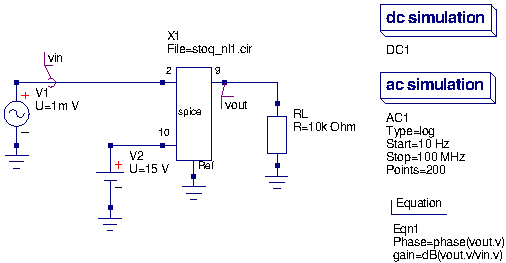
\includegraphics[width=0.6\linewidth]{stoq_fig2}
  \caption{Qucs schematic for the two stage amplifier represented by the SPICE netlist shown in Fig.~\ref{fig:stoq_fig1}.}
  \label{fig:stoq_fig2}
\end{figure} 
\FloatBarrier




\begin{figure}
  \centering
  \begin{lstlisting} [
    basicstyle=\scriptsize]
.Def:stoq_nl1_cir _net2 _net9 _net10 _ref
  C:C3 _net7 _net9 C="10uF"
  C:C5 _net8 _ref C="25uF"
  R:R8 _net8 _ref R="3.6k"
  BJT:Q2 _net6 _net7 _net8 _ref Type="npn" Is="2e-16" Bf="50" Br="1" 
      Rb="5" Rc="1" Re="0" Cje="0.4pF"Vje="0.8" Mje="0.4" Cjc="0.5pF" 
      Vjc="0.8" Cjs="1pF" Vaf="100" Nf="1" Nr="1" Ikf="0" Ikr="0" Var="0"
      Ise="0" Ne="1.5" Isc="0" Nc="2" Rbm="0" Irb="0" Mjc="0.33" Xcjc="1" 
      Vjs="0.75" Mjs="0" Fc="0.5" Vtf="0" Tf="0" Xtf="0" Itf="0" Tr="0"
  R:R7 _net10 _net7 R="6.8k"
  R:R4 _net6 _ref R="30k"
  R:R3 _net10 _net6 R="120k"
  C:C4 _net5 _ref C="15uF"
  C:C2 _net4 _net6 C="10uF"
  R:R6 _net5 _ref R="3.6k"
  BJT:Q1 _net3 _net4 _net5 _ref Type="npn" Is="2e-16" Bf="50" Br="1"
      Rb="5" Rc="1" Re="0" Cje="0.4pF"Vje="0.8" Mje="0.4" Cjc="0.5pF" 
      Vjc="0.8" Cjs="1pF" Vaf="100" Nf="1" Nr="1" Ikf="0" Ikr="0" Var="0"
      Ise="0" Ne="1.5" Isc="0" Nc="2" Rbm="0" Irb="0" Mjc="0.33" Xcjc="1" 
      Vjs="0.75" Mjs="0" Fc="0.5" Vtf="0" Tf="0" Xtf="0" Itf="0" Tr="0"
  R:R5 _net10 _net4 R="12k"
  R:R2 _net3 _ref R="50k"
  R:R1 _net3 _net10 R="200k"
  C:C1 _net2 _net3 C="10uF"
.Def:End
\end{lstlisting} 
  \caption{Qucs format netlist for the two stage BJT amplifier: NOTE -In this listing the entries for Q1 and Q2 have been edited so that they fit on the text page.}
  \label{fig:stoq_fig3}
\end{figure} 


\begin{figure}
  \centering
  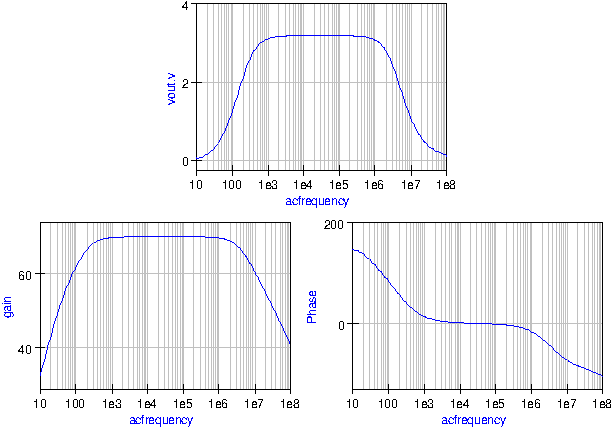
\includegraphics[width=1.0\linewidth]{stoq_fig4}
  \caption{Simulation waveforms for the two stage amplifier.}
  \label{fig:stoq_fig4}
\end{figure} 



\tutsection{Defining symbols for Qucs SPICE netlist components}

Qucs automatically generates the symbol for a SPICE netlist component and does not allow users to edit the resulting symbol. One of the disadvantage of this feature is that the placement of the symbol input and output pins may be in a position which is contrary to accepted use or signal flow direction. To overcome this limitation a user defined symbol may be constructed where the SPICE netlist component is embedded within the new symbol. Figure~\ref{fig:stoq_fig5} illustrates such a symbol for the two stage BJT amplifier and the resulting Qucs netlist for the new symbol is shown in Fig.~\ref{fig:stoq_fig6}. From Fig.~\ref{fig:stoq_fig6} we observe that embedding a SPICE netlist symbol, within a user defined symbol, introduces an additional subcircuit call in the resulting Qucs netlist; this is probably a small price to pay for the convenience that a user defined symbol brings to the overall simulation process.\begin{figure}
  \centering
  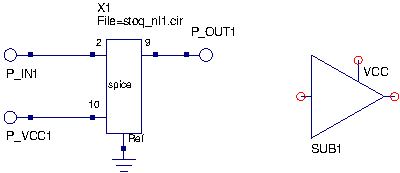
\includegraphics[width=0.6\linewidth]{stoq_fig5}
  \caption{User defined symbol for the two stage BJT amplifier. }
  \label{fig:stoq_fig5}
\end{figure} 



\begin{figure}
  \centering
  \begin{lstlisting} [
    basicstyle=\scriptsize]
  
.Def:stoq_fig5_amp _net0 _net1 _net2
Sub:X1 _net0 _net1 _net2 gnd Type="stoq_nl1_cir"
.Def:End

.Def:stoq_nl1_cir _net2 _net9 _net10 _ref
  C:C3 _net7 _net9 C="10uF"
  C:C5 _net8 _ref C="25uF"
  R:R8 _net8 _ref R="3.6k"
  BJT:Q2 _net6 _net7 _net8 _ref Type="npn" Is="2e-16" Bf="50" Br="1" 
      Rb="5" Rc="1" Re="0" Cje="0.4pF"Vje="0.8" Mje="0.4" Cjc="0.5pF" 
      Vjc="0.8" Cjs="1pF" Vaf="100" Nf="1" Nr="1" Ikf="0" Ikr="0" Var="0"
      Ise="0" Ne="1.5" Isc="0" Nc="2" Rbm="0" Irb="0" Mjc="0.33" Xcjc="1" 
      Vjs="0.75" Mjs="0" Fc="0.5" Vtf="0" Tf="0" Xtf="0" Itf="0" Tr="0"
  R:R7 _net10 _net7 R="6.8k"
  R:R4 _net6 _ref R="30k"
  R:R3 _net10 _net6 R="120k"
  C:C4 _net5 _ref C="15uF"
  C:C2 _net4 _net6 C="10uF"
  R:R6 _net5 _ref R="3.6k"
 BJT:Q1 _net3 _net4 _net5 _ref Type="npn" Is="2e-16" Bf="50" Br="1"
      Rb="5" Rc="1" Re="0" Cje="0.4pF"Vje="0.8" Mje="0.4" Cjc="0.5pF" 
      Vjc="0.8" Cjs="1pF" Vaf="100" Nf="1" Nr="1" Ikf="0" Ikr="0" Var="0"
      Ise="0" Ne="1.5" Isc="0" Nc="2" Rbm="0" Irb="0" Mjc="0.33" Xcjc="1" 
      Vjs="0.75" Mjs="0" Fc="0.5" Vtf="0" Tf="0" Xtf="0" Itf="0" Tr="0"
  R:R5 _net10 _net4 R="12k"
  R:R2 _net3 _ref R="50k"
  R:R1 _net3 _net10 R="200k"
  C:C1 _net2 _net3 C="10uF"
.Def:End
\end{lstlisting}
  \caption{Qucs format netlist for the two stage BJT amplifier represented by a user defined symbol: NOTE -In this listing the entries for Q1 and Q2 have been edited so that they fit on the text page.}
  \label{fig:stoq_fig6}
\end{figure} 

\tutsection{Handling SPICE subcircuits}

Although Qucs treats SPICE netlist components as subcircuits the SPICE to Qucs netlist conversion process still allows SPICE subcircuits to be defined within the SPICE file being converted.  Such subcircuits then become local subcircuits to the SPICE netlist component to which they are attached.  This allows complex circuits consisting of many related, but often different, circuit blocks to be represented by a single symbol in a Qucs schematic.  In such cases the resulting symbol represents a true subsection of an entire circuit rather than a simple single circuit function subcircuit. To demonstrate this feature consider the following examples; (1) a multisection LC delay line and (2) a CMOS ring counter.

\tutsubsection{Subcircuit example 1: a multisection LC delay line}
The SPICE netlist for a ten section LC passive delay line is shown in Fig.~\ref{fig:stoq_fig7}. In this listing each LC delay section is represented by a SPICE subcircuit and these sections are connected in series to form the overall delay line.  Figures~\ref{fig:stoq_fig8} and ~\ref{fig:stoq_fig9} present the resulting Qucs netlist and generated waveforms obtained with the test circuit shown in Fig.~\ref{fig:stoq_fig10}.


\begin{figure}
 \begin{lstlisting} [
    basicstyle=\scriptsize]
* Z0 = 320 Ohm.
*
.subckt lc n1 n2
l1 n1 n2 10uh
c1 n2 0 10pf
.ends
*
rs n9 n10 320ohm
x1 n10 n11 lc
x2 n11 n12 lc
x3 n12 n13 lc
x4 n13 n14 lc
x5 n14 n15 lc
x6 n15 n16 lc
x7 n16 n17 lc
x8 n17 n18 lc
x9 n18 n19 lc
x10 n19 n20 lc
rl n20 0 320ohm
.end
\end{lstlisting} 
  \caption{SPICE netlist for a ten section LC delay line..}
  \label{fig:stoq_fig7}
\end{figure} 



\begin{figure}
 \begin{lstlisting} [
    basicstyle=\scriptsize]
.Def:stoq_fig10a _net0 _net10 _net1 _net2 _net3 _net4 
                 _net5 _net6 _net7 _net8 _net9
Sub:X1 _net0 _net10 _net1 _net2 _net3 _net4 
             _net5 _net6 _net7 _net8 _net9 gnd Type="test3_pp_cir"
.Def:End

.Def:test3_pp_cir _netN9 _netN11 _netN12 _netN13 _netN14 
                 _netN15 _netN16 _netN17 _netN18 _netN19 _netN20 _ref
  R:RL _netN20 _ref R="320Ohm"
  Sub:X10 _ref _netN19 _netN20 Type="LC"
  Sub:X9 _ref _netN18 _netN19 Type="LC"
  Sub:X8 _ref _netN17 _netN18 Type="LC"
  Sub:X7 _ref _netN16 _netN17 Type="LC"
  Sub:X6 _ref _netN15 _netN16 Type="LC"
  Sub:X5 _ref _netN14 _netN15 Type="LC"
  Sub:X4 _ref _netN13 _netN14 Type="LC"
  Sub:X3 _ref _netN12 _netN13 Type="LC"
  Sub:X2 _ref _netN11 _netN12 Type="LC"
  Sub:X1 _ref _netN10 _netN11 Type="LC"
  R:RS _netN9 _netN10 R="320Ohm"
  .Def:LC _ref _netN1 _netN2
  L:L1 _netN1 _netN2 L="10uH"
  C:C1 _netN2 _ref C="10pF"
  .Def:End
.Def:End
\end{lstlisting} 
  \caption{Qucs netlist for a 10 section LC delay line: NOTE -In this listing the entries for the .Def statements have been edited so that they fit on the text page.}
  \label{fig:stoq_fig8}
\end{figure} 

\begin{figure}
  \centering
  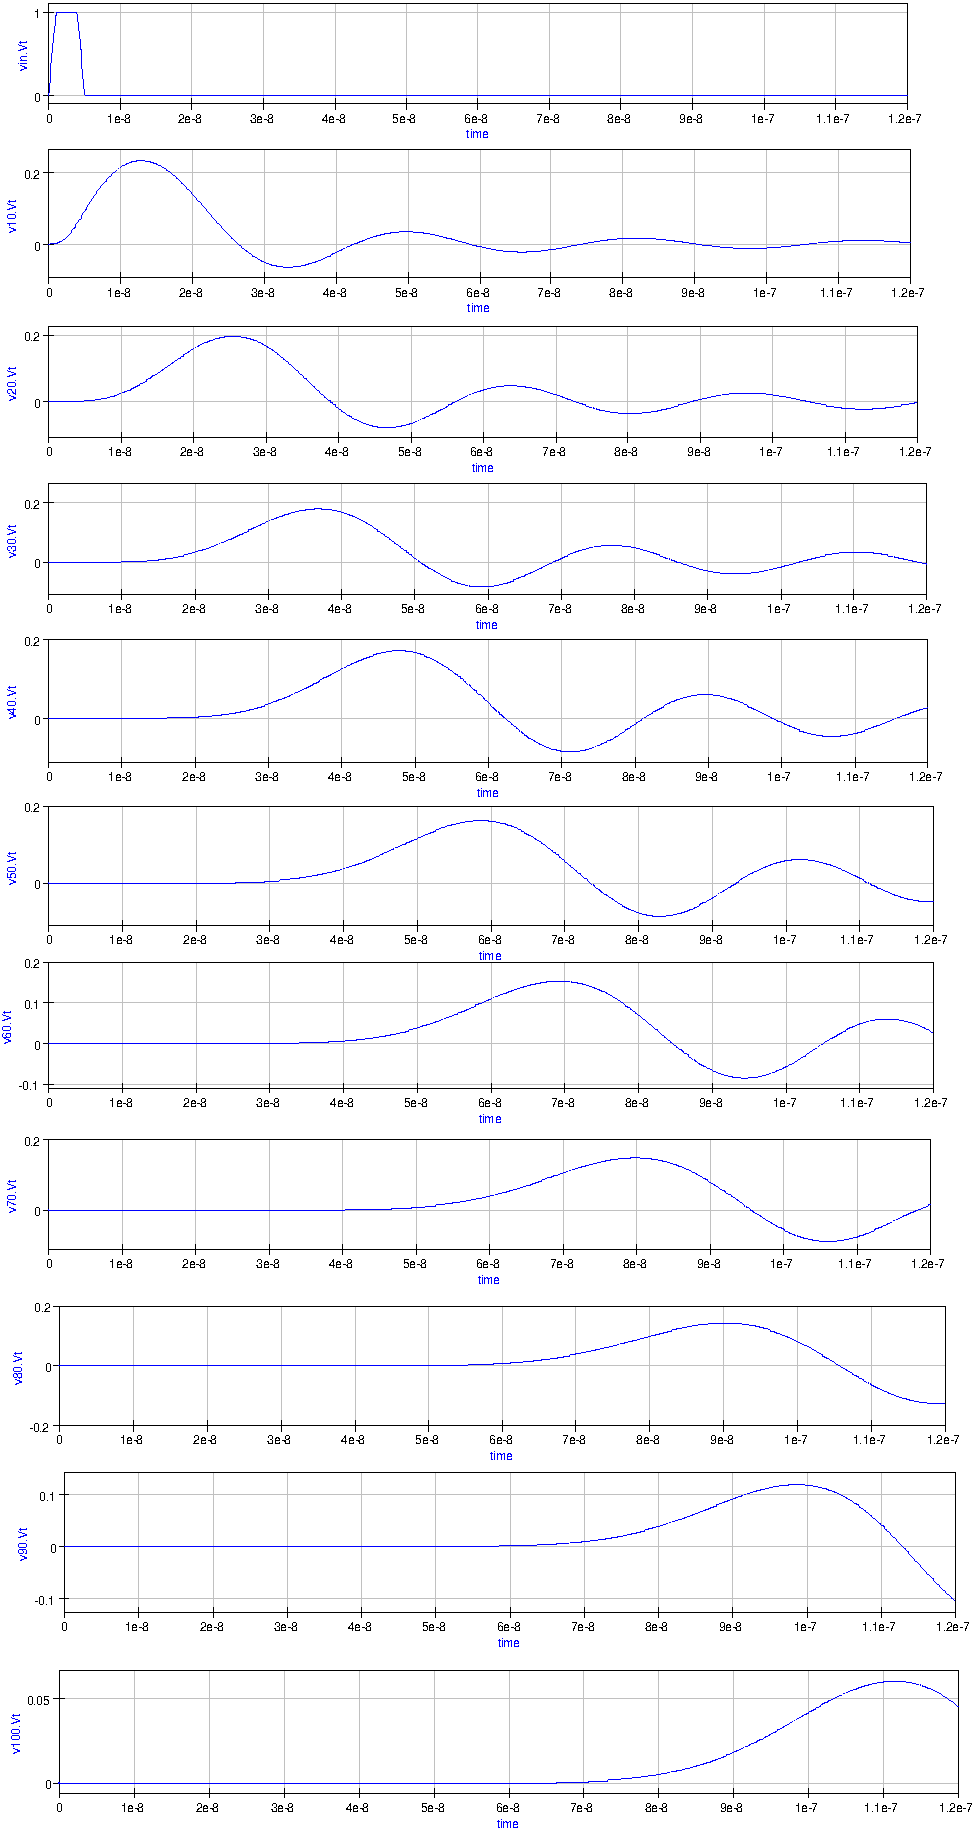
\includegraphics[width=0.7\linewidth]{stoq_fig9}
  \caption{Simulation waveforms for a 10 section LC delay line.}
  \label{fig:stoq_fig9}
\end{figure} 

\begin{figure}
  \centering
  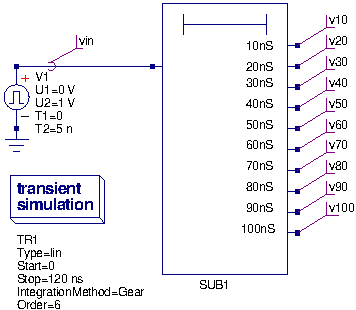
\includegraphics[width=0.5\linewidth]{stoq_fig10}
  \caption{LC delay line test circuit.}
  \label{fig:stoq_fig10}
\end{figure} 

\tutsubsection{Subcircuit example 2: a two section CMOS ring counter}
Subcircuit example one only contains a single local subcircuit. The next example demonstrates how SPICE listings with more than one subcircuit are handled by Qucs.  Such circuits are representative of more complex electronic systems which form easily identifiable subsystem blocks.\footnote{One significant advantage that Qucs has when compared to netlist entry only circuit simulators is that it is possible the define schematic symbols for subsystem blocks that comprise discreet components and one or more local subcircuits. These may then be employed like any other Qucs symbols when constructing circuit schematics.} Fig.~\ref{fig:stoq_fig11} shows the SPICE netlist for a simple two section CMOS ring counter. This circuit is modelled at discreet component level and uses basic level one MOS parameters to define the MOS transistors. These are then combined to form NAND and NOR subcircuits. Again for completeness the resulting Qucs netlist is shown in Fig.~\ref{fig:stoq_fig12} together with a typical set of counter input and output signal waveforms, Fig.~\ref{fig:stoq_fig13}.

\begin{figure}
 \begin{lstlisting} [
   basicstyle=\scriptsize]   
* Two stage CMOS ring counter circuit.
*
x1 1 5 6  nand2
x2 1 6 7  nand2
x3 3 6 2  nand2
x4 2 7 3  nand2
x5 1 2 8  nor2
x6 1 8 9  nor2
x7 5 8 4  nor2
x8 4 9 5  nor2
*
.model modp pmos( vto=-1 kp=10u
+                         cgdo=0.2n cgso=0.2n cgbo=2n)
.model modn nmos(vto=1 kp=10u
+                         cgdo=0.2n cgso=0.2n cgbo=2n)
*
.subckt nand2 1 2 3 
m1 3 1 4 4 modp w=40u l=5u
m2 3 2 4 4 modp w=40u l=5u
m3 5 1 0 0 modn w=20u l=5u
m4 3 2 5 5 modn w=20u l=5u
c1 1 0 10p
c2 2 0 10p
vcc 4 0 pulse ( 0 5 0 1ns 1ns 1 2)
.ends
*
.subckt nor2 1 2 3
m1 4 1 7 7 modp w=40u l=5u
m2 3 2 4 4 modp w=40u l=5u
m3 3 2 0 0 modn w=20u l=5u
m4 3 1 0 0 modn w=20u l=5u
c1 1 0 10p
c2 2 0 10p
vcc 7 0 pulse ( 0 5 0 1ns 1ns 1 2)
.ends
.end
\end{lstlisting} 
 \caption{SPICE netlist for a two section CMOS ring counter.}
\label{fig:stoq_fig11}
\end{figure}   

\begin{figure}

 \begin{lstlisting} [
   basicstyle=\scriptsize]   
# Qucs 0.0.11  /media/hda2/OPAMP_templates/test_stoq_fig11a.sch
.Def:stoq_fig11a_cir _net1 _net4 _ref
  .Def:NOR2 _ref _net1 _net2 _net3
  Vpulse:VCC _net7 _cnet0 U1="0" U2="5" T1="0" Tr="1ns" Tf="1ns" T2="1"
  MOSFET:M1 _net1 _net4 _net7 _net7 Type="pfet" W="40u" L="5u" Vt0="-1" 
         Kp="10u" Cgdo="0.2n" Cgso="0.2n" Cgbo="2n" Is="1e-14" N="1" 
         Lambda="0" Gamma="0" Phi="0.6"
  MOSFET:M2 _net2 _net3 _net4 _net4 Type="pfet" W="40u" L="5u" Vt0="-1" 
         Kp="10u" Cgdo="0.2n" Cgso="0.2n" Cgbo="2n" Is="1e-14" N="1" 
         Lambda="0" Gamma="0" Phi="0.6"
  MOSFET:M3 _net2 _net3 _ref _ref Type="nfet" W="20u" L="5u" Vt0="1" 
         Kp="10u" Cgdo="0.2n" Cgso="0.2n" Cgbo="2n" Is="1e-14" N="1" 
         Lambda="0" Gamma="0" Phi="0.6"
  MOSFET:M4 _net1 _net3 _ref _ref Type="nfet" W="20u" L="5u" Vt0="1" 
         Kp="10u" Cgdo="0.2n" Cgso="0.2n" Cgbo="2n" Is="1e-14" N="1" 
         Lambda="0" Gamma="0" Phi="0.6"
  C:C1 _net1 _ref C="10p"
  C:C2 _net2 _ref C="10p"
  Vdc:VCC _cnet0 _ref U="0"
  .Def:End
  .Def:NAND2 _ref _net1 _net2 _net3
  Vpulse:VCC _net4 _cnet1 U1="0" U2="5" T1="0" Tr="1ns" Tf="1ns" T2="1"
  MOSFET:M1 _net1 _net3 _net4 _net4 Type="pfet" W="40u" L="5u" Vt0="-1" 
         Kp="10u" Cgdo="0.2n" Cgso="0.2n" Cgbo="2n" Is="1e-14" N="1" 
         Lambda="0" Gamma="0" Phi="0.6"
  MOSFET:M2 _net2 _net3 _net4 _net4 Type="pfet" W="40u" L="5u" Vt0="-1" 
         Kp="10u" Cgdo="0.2n" Cgso="0.2n" Cgbo="2n" Is="1e-14" N="1" 
         Lambda="0" Gamma="0" Phi="0.6"
  MOSFET:M3 _net1 _net5 _ref _ref Type="nfet" W="20u" L="5u" Vt0="1" 
         Kp="10u" Cgdo="0.2n" Cgso="0.2n" Cgbo="2n" Is="1e-14" N="1" 
         Lambda="0" Gamma="0" Phi="0.6"
  MOSFET:M4 _net2 _net3 _net5 _net5 Type="nfet" W="20u" L="5u" Vt0="1" 
         Kp="10u" Cgdo="0.2n" Cgso="0.2n" Cgbo="2n" Is="1e-14" N="1" 
         Lambda="0" Gamma="0" Phi="0.6"
  C:C1 _net1 _ref C="10p"
  C:C2 _net2 _ref C="10p"
  Vdc:VCC _cnet1 _ref U="0"
  .Def:End
  Sub:X8 _ref _net4 _net9 _net5 Type="NOR2"
  Sub:X7 _ref _net5 _net8 _net4 Type="NOR2"
  Sub:X6 _ref _net1 _net8 _net9 Type="NOR2"
  Sub:X5 _ref _net1 _net2 _net8 Type="NOR2"
  Sub:X4 _ref _net2 _net7 _net3 Type="NAND2"
  Sub:X3 _ref _net3 _net6 _net2 Type="NAND2"
  Sub:X2 _ref _net1 _net6 _net7 Type="NAND2"
  Sub:X1 _ref _net1 _net5 _net6 Type="NAND2"
.Def:End
Sub:X1 vin vout gnd Type="stoq_fig11a_cir"
Vrect:V1 vin gnd U="5 V" TH="1 us" TL="1 us" Tr="1 ns" Tf="1 ns" Td="0 ns"
.TR:TR1 Type="lin" Start="0" Stop="30u" Points="1000" IntegrationMethod="Trapezoidal" 
Order="2" InitialStep="0.01 ns" MinStep="1e-18" MaxIter="150" reltol="0.01" 
abstol="1 uA" vntol="100 uV" Temp="26.85" LTEreltol="1e-3" LTEabstol="1e-4" 
LTEfactor="1" Solver="CroutLU" relaxTSR="no" initialDC="yes" MaxStep="0"

\end{lstlisting} 
 \caption{Qucs netlist for a two section CMOS ring counter: NOTE -In this listing the entries for MOSFETs and transient analysis have been edited so that they fit on the text page.}
\label{fig:stoq_fig12}
\end{figure}   

\begin{figure}
  \centering
  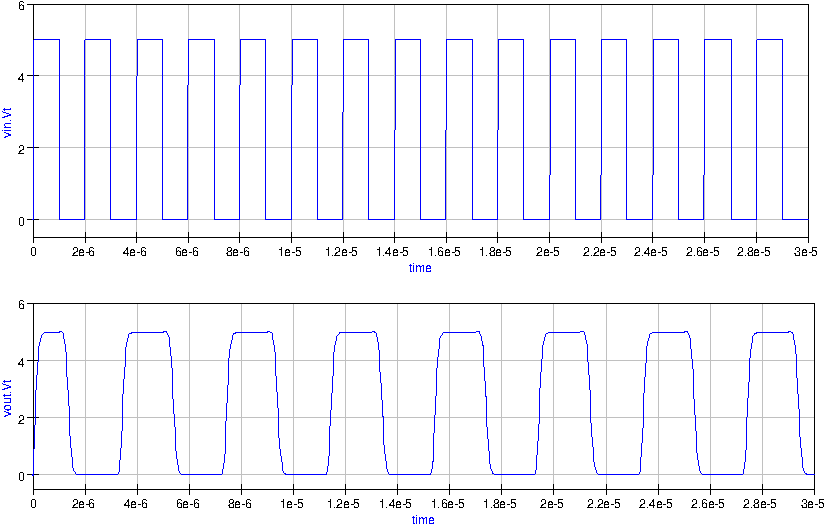
\includegraphics[width=1.0\linewidth]{stoq_fig13}
  \caption{Two stage CMOS ring counter signal waveforms.}
  \label{fig:stoq_fig13}
\end{figure} 

\tutsection{Limitations when converting SPICE netlists}
Not all SPICE netlists can be converted to Qucs netlist format and simulated by Qucs\footnote{A number of Qucs users have reported problems in the past when trying to simulate SPICE netlists for components that have been published by device manufactures, see for example, "Qucs SPICE error - please...", William Flyn <WF215@ca...>, 29.8.2006, Qucs help forum. }.  There are a number of reasons for this.  The first and most obvious is due to the fact that some SPICE components have not been implemented in Qucs yet.  Nonlinear controlled voltage and current sources are an example.\footnote{SPICE 2 polynomal controlled voltage and current sources and SPICE 3 type B sources are not implemented in any of the Qucs versions so far released. Their implementation is on the to-do list but no date for their implementation has been fixed yet. }  There are also a number of detailed differences between the SPICE and Qucs implementation of components common to both simulators, one being the lack of PWL features in the Qucs independent voltage and current sources. A second area that represents a significant limitation, for those readers who regularly write SPICE netlists as part of their simulation work, is the fact that Qucs contains a much greater range of predefined primitive components that are not available in either the SPICE 2 or SPICE 3 simulators.  Perhaps this is not so much a limitation but an indication of the current development effort being put into Qucs by the development team. As the development of Qucs progresses it is expected that all the component features found in SPICE will have a corresponding entry in Qucs\footnote{Future plans in this area are discussed in a later section of these notes.}. 

\tutsection{Extending the SPICE netlist language}
The standard SPICE 2 and SPICE 3 hardware description languages do not allow (1) component values to be defined by algebraic equations\footnote{Please note this is not strictly true as SPICE 3 B sources can be defined by equations involving simulation variables and other data.} or (2) parameters to be passed to subcircuits. This makes writing universal subcircuit models very difficult, forcing semiconductor device manufacturers to issue individual SPICE models for each device they manufacture rather than a single generalised model\footnote{In a generalised model only one model description is provided for each generic component/circuit. Different component models are formed by passing parameters to the generalised model.  SPICE employs this approach to represent semiconductor devices through the use of the .model statement.  However, in the .model case the code for each type of semiconductor device is hardwired into the simulator code rather than being defined by a subcircuit.} for a given type of integrated circuit. A well known example being the SPICE Boyle\footnote{Boyle,G.R., B.M. Cohn, D.O. Pederson, and J.E. Solomon, 1974, Macromodeling of integrated circuit amplifiers, IEEE Journal of Solid-State Circuits (December).} operational amplifier models. A number of current commercial circuit simulators\footnote{For example PSPICE, HSPICE and IS-SPICE.} have been extended to include the parameter based features outlined above. In the case of those simulators based on the unextended Berkely SPICE 2G6 or SPICE 3F5\footnote{For example NGSPICE, TCLSPICE and WINSPICE.} code a different approach is often adopted. This is based on the use of a preprocessor, similar to that found in the C language, which takes as input a parameter and equation style netlist and outputs a standard SPICE netlist with the parameters and equations evaluated to give a numerical result.  The advantage of this approach is that the preprocessor can be used with any SPICE simulator or indeed with Qucs. Two such preprocessors are SPICEPRM and SPICEPP.\footnote{(1) Andrew J. Borsa, SPICEPRM, A SPICE preprocessor for parameterised subcircuits, V 0.11, 1996, <andy@moose.mv.com> (SPICEPRM can be downloaded from the Sourceforge.net ngspice project.) and (2) John Shaehen, SPICEPP, A SPICE proprocessor for SPICE 3F5, V 1.5, 2000, <john@reptechnic.com.au>. (SPICEPP can be downloaded from the Sourceforge.net tclspice project.)}  The flow diagram for the Qucs simulation sequence including a SPICE preprocessing stage is shown in Fig.~\ref{fig:stoq_fig14}. This diagram clearly shows how both standard SPICE and parameterised netlists can be linked into the Qucs simulation cycle. Of the two SPICE preprocessors introduced above SPICEPP is probably the most useful from a Qucs users point of view\footnote{SPICEPP was written after SPICEPRM and extends the facilities offered by SPICEPRM. } as it adds more features to the overall simulation process. Hence the notes that follow will concentrate on describing how SPICEPP can be used with Qucs.

\tutsubsection{The SPICEPP preprocessor}
SPICEPP\footnote{SPICEPP is written in PERL. The SPICEPP.pl script should be copied to a directory on your search path. On my system I keep it in the Qucs bin directory. PERL must also be installed on your system.} is a preprocessor for Berkeley SPICE 3F5, adding support for a number of structures found in commercial SPICE simulators, specifically SPICE commands .param, .global, .lib, .temp, .meas and inline comments \verb|($)|. The remainder of these notes explain the use of commands .param, .global and the inline comment as these add specific functionality to Qucs that is not provided by other sections of the Qucs simulation software. The definition of these commands are:
\begin{itemize}
\item .param data=dataval <data2=dataval2> ............ 
The .param statement adds the ability to parameterise SPICE data, including component values, voltages, currents and equations.
\item .globel node1 <node2> ...............
The .global statement causes the named nodes to override local subcircuit nodes of the same name.
\item Algebraic statements are enclosed in quotes `        `\footnote{The ` character can be found on the most left key on the row of numerical keys (` 1 2 3 4 5 6 7 8 9 0 - .......) - this is the case on my keyboard.}.
\item Inline comments start with the \verb|$| symbol and continue to the end of a line.
\end{itemize}

  


 

\begin{figure}
  \centering
  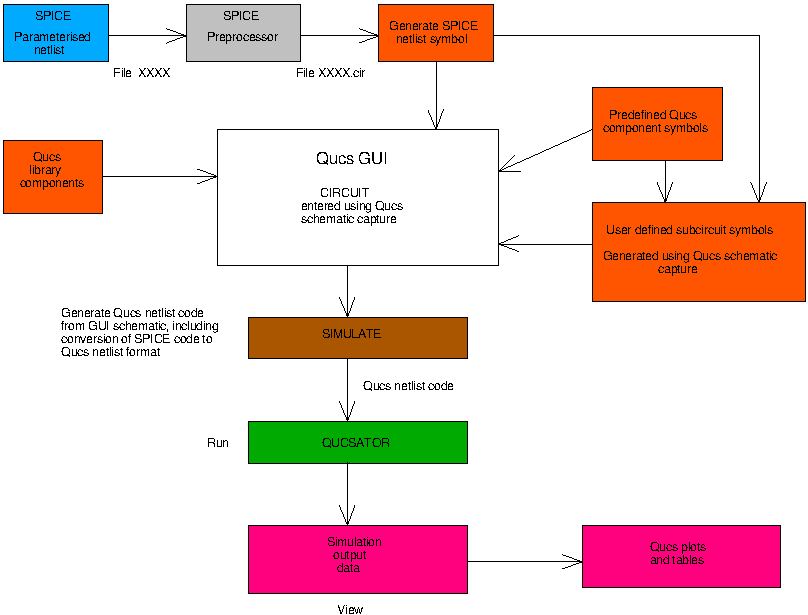
\includegraphics[width=1.0\linewidth]{stoq_fig14}
  \caption{Flow diagram of Qucs simulator stages including SPICE preprocessing.}
  \label{fig:stoq_fig14}
\end{figure} 

\tutsection{Circuit template models}
When modelling devices or circuits for simulation a particularly productive approach is the use of a universal template that can be employed to generate models for devices of the same type but with different characteristics.  By simply changing the parameters embedded in a universal template a new device model is generated when the netlist code is passed through the SPICEPP preprocessor.  Consider the SPICE template model shown in Fig.~\ref{fig:stoq_fig15}. This represents a simple modular AC macromodel\footnote{Details of the model derivation can be found in the Qucs Modelling Operational Amplifiers tutorial, Qucs Web site.} for an OP AMP. OP AMP internal pins are given by integers and external pins by names in SPICE 3 format. The parameters for a UA741 OP AMP are shown listed at the start of the SPICE preprocessor netlist. These are used in the calculation of the component values in later sections of the netlist.  In all cases parameters must be defined before they are used in component calculations.  Passing this listing through the SPICEPP preprocessor\footnote{The SPICEPP PERL script can be run from a shell using the command \textbf{\textit{spicepp.pl name.pp > name.cir}}, where name is the name of the file to be processed.} and generating a Qucs user defined symbol for the UA741 OP AMP results in the Qucs netlist and symbol shown in Figures~\ref{fig:stoq_fig16} and~\ref{fig:stoq_fig17}. An application of the generated UA741 OP AMP model is shown in Fig.~\ref{fig:stoq_fig18}.  This circuit is a notch filter. In Fig.~\ref{fig:stoq_fig18} the band rejection characteristic of the filter are realised by a twin-T RC network. Figure~\ref{fig:stoq_fig19} shows the simulated small signal transfer characteristics of this filter.  

\begin{figure}
 \begin{lstlisting} [
   basicstyle=\scriptsize]   
*
* Device pins 1. input  in_n, in_p
*             2. output out
*
* ua741 OP AMP parameters
*
.param voff = 0.7m
.param ib = 80n
.param ioff = 20n
.param rd = 2meg
.param cd = 1.4p 
.param cmrrdc = 31622.8
.param fcmz = 200.0
.param aoldc = 199526
.param gbp = 1meg
.param fp2 = 3meg
.param ro = 75.0
*
* input stage 
*
voff1 in_n 6 'voff/2'
voff2 7 in_p 'voff/2'
ib1   0 6 ib
ib2   7 0 ib
ioff1 7 6 'ioff/2'
r1    6 8 'rd/2'
r2    7 8 'rd/2'
cin1  6 7 cd
*
* common-mode zero stage
*
ecm1 12 0 8 0 '1e6/cmrrdc'
rcm1 12 13 1meg
ccm1 12 13 '1/(2 * 3.1412 * 1e6 * fcmz)'
rcm2 13 0 1
*
* differential and common-mode
* signal summing stage
*
gmsum1 0 14 7 6 1
gmsum2 0 14 13 0 1
rsum1  14 0 1
*
* voltage gain stage 1 
*
gmp1 0 9 14 0 1
rado 9 0 aoldc
cp1 9 0 '1/(2 * 3.1412 * gbp)'
*
* voltage gain stage 2 
*
gmp2 0 11 9 0 1
rp2  11 0 1
cp2  11 0 '1/(2 * 3.1412 * fp2)'
*
* output stage 
*
eos1 10 0 11 0 1
ros1 10 out ro
*
\end{lstlisting} 
 \caption{SPICE template preprocessor netlist for a UA741 AC modular OP AMP model.}
\label{fig:stoq_fig15}
\end{figure}   

\begin{figure}
 \begin{lstlisting} [
   basicstyle=\scriptsize]   
.Def:stoq_fig17 _net0 _net1 _net2
Sub:X1 _net0 _net1 _net2 gnd Type="stoq_fig15_cir"
.Def:End

.Def:stoq_fig15_cir _netIN_N _netOUT _netIN_P _ref
  R:ROS1 _net10 _netOUT R="75"
  VCVS:EOS1 _net11 _net10 _ref _ref G="1"
  C:CP2 _net11 _ref C="5.30583e-08"
  R:RP2 _net11 _ref R="1"
  VCCS:GMP2 _net9 _ref _net11 _ref G="1"
  C:CP1 _net9 _ref C="1.59175e-07"
  R:RADO _net9 _ref R="199526"
  VCCS:GMP1 _net14 _ref _net9 _ref G="1"
  R:RSUM1 _net14 _ref R="1"
  VCCS:GMSUM2 _net13 _ref _net14 _ref G="1"
  VCCS:GMSUM1 _net7 _ref _net14 _net6 G="1"
  R:RCM2 _net13 _ref R="1"
  C:CCM1 _net12 _net13 C="7.95874e-10"
  R:RCM1 _net12 _net13 R="1M"
  VCVS:ECM1 _net8 _net12 _ref _ref G="31.6228"
  C:CIN1 _net6 _net7 C="1.4e-12"
  R:R2 _net7 _net8 R="1e+06"
  R:R1 _net6 _net8 R="1e+06"
  Idc:IOFF1 _net7 _net6 I="1e-08"
  Idc:IB2 _net7 _ref I="8e-08"
  Idc:IB1 _ref _net6 I="8e-08"
  Vdc:VOFF2 _net7 _netIN_P U="0.00035"
  Vdc:VOFF1 _netIN_N _net6 U="0.00035"
.Def:End

\end{lstlisting} 
 \caption{Qucs netlist for a UA741 AC modular OP AMP model.}
\label{fig:stoq_fig16}
\end{figure}   

\begin{figure}
  \centering
  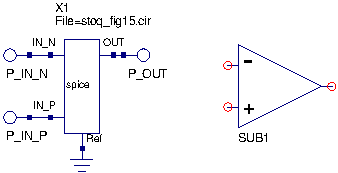
\includegraphics[width=0.7\linewidth]{stoq_fig17}
  \caption{Qucs symbol for a UA741 AC modular OP AMP model.}
  \label{fig:stoq_fig17}
\end{figure} 

\begin{figure}
  \centering
  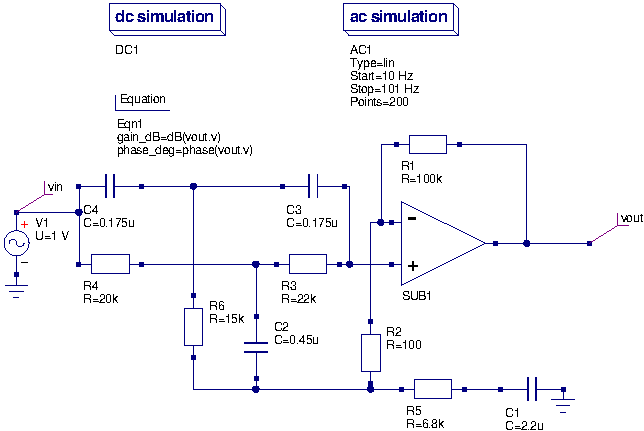
\includegraphics[width=0.7\linewidth]{stoq_fig18}
  \caption{A twin-T notch filter circuit.}
  \label{fig:stoq_fig18}
\end{figure} 

\begin{figure}
  \centering
  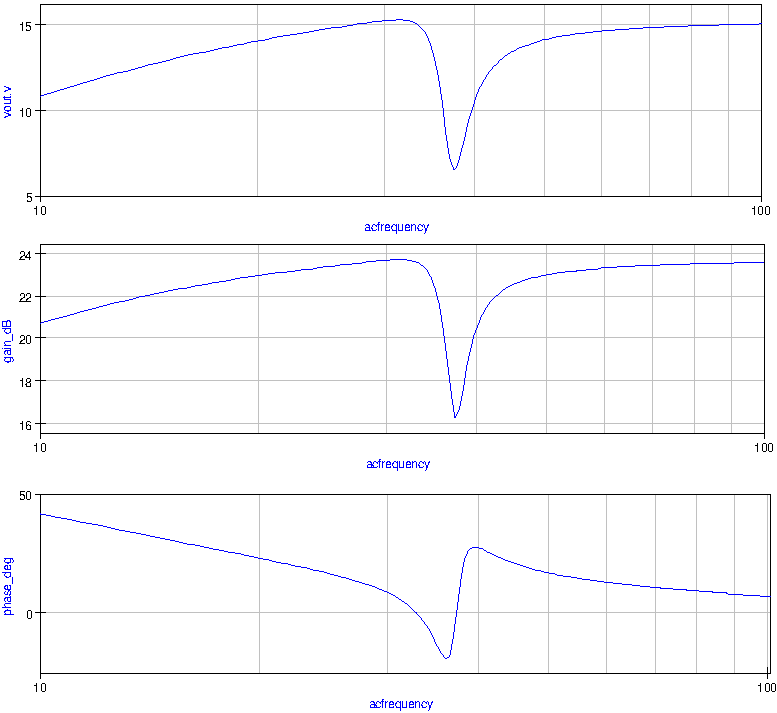
\includegraphics[width=0.7\linewidth]{stoq_fig19}
  \caption{Small signal transfer characteristics for a twin-T notch filter circuit.}
  \label{fig:stoq_fig19}
\end{figure} 

\tutsection{Building circuit design equations into netlists}
Figure~\ref{fig:stoq_fig20} illustrates a bandpass filter that has a bandwidth which is small compared to it's center frequency.  The circuit is often referred to as the Dalyiannis-Friend filter after its developers. The filter center frequency $f_{0}$, voltage gain magnitude $H_{0}$, bandwidth B and Q factor are given by the following equations:

\begin{itemize}
\item $f_{0}=\dfrac{1}{2 \pi C\sqrt{(R_{1} \Vert R_{2}) R_{3}}}$, where $C = C_{1} = C_{2}$
\item $H_{0} = \dfrac{R_{3}}{2 R_{1}}$
\item $B=\dfrac{1}{\pi R_{3} C}$ 
\item $Q=\dfrac{f_{0}}{B} = \dfrac{1}{2} \sqrt{\dfrac{R_{3}}{R_{1} \Vert R_{2}}}$
\end{itemize}

When designing a filter for a specific specification, for example say $f_{0}=1kHz$, $B=200Hz$ and $H_{0}=10$, values for the filter resistor and capacitor values need to be calculated.  This can, of course, be done manually. However, this process is often tedious, especially if a number of filters need to be designed each with different specifications.  Circuit simulators are by their very nature primarily designed to analyse and simulate the performance of circuits who's component values are known.  As such they are tools for analysis rather than design.  In practice, of course, engineers employ circuit simulators to check their circuit designs.  Qucs is attempting to bridge the gap between design and analysis by using add-on software components for designing circuits with well understood structures and design procedures\footnote{The Qucs Tools drop-down menu lists the currently available design functions that have been implemented with release of Qucs you are using.}.

\begin{figure}
  \centering
  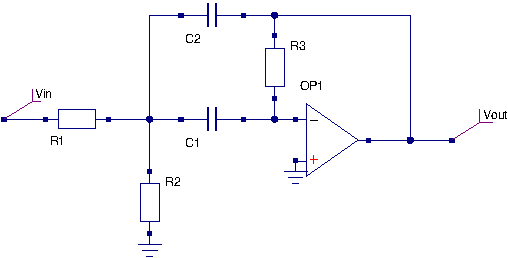
\includegraphics[width=0.6\linewidth]{stoq_fig20}
  \caption{The Dalyiannis-Friend bandpass filter circuit.}
  \label{fig:stoq_fig20}
\end{figure} 

In the previous section it was shown that the SPICEPP preprocessor could be used to calculate model component values.  By a simple extension of this concept it is also possible to embed design equations into a netlist.  Shown in Fig.~\ref{fig:stoq_fig21} is a SPICEPP netlist for the Dalyiannis-Friend filter. The UA741 OP AMP is modelled with a SPICE subcircuit called \verb|opamp_ac| and has its own set of parameters\footnote{These are defined within a subcircuit and should have names unique to the subcircuit model being defined.}. The first set of design parameters represent the filter specification and are used in the SPICEPP conversion process to calculate the filter resistor and capacitor component values.  Note also the use of inline comments for documenting the netlist code. Figures.~\ref{fig:stoq_fig22} and~\ref{fig:stoq_fig23} show a basic filter test circuit and the resulting simulation transfer functions. Hence, not only can the SPICEPP preprocessor be used for setting up device models but it can also aid the design of entire circuit blocks provided design equations are available for a given circuit configuration. By combining SPICEPP with Qucs a very significant design/analysis tool becomes available opening up new possibilities for Qucs users.  

\begin{figure}
 \begin{lstlisting} [
   basicstyle=\scriptsize]   
* Delyiannis Friend Bandpass filter design
* Design parameters
.param fc =   2000.0    $ Filter center frequency (Hz)
.param bw  =  200.0     $ Filter bandwidth (Hz)
.param q   =  10.0      $ Filter q factor = f0/bw
.param r3iv = 200k      $ Assumed value for rf3
.param h0 =   10.0      $ Filter f0 gain magnitude
*
* Filter circuit pins: input n1, output n3
*
r3 n3 n4  r3iv
c1 n2 n3 'q/(3.1412*fc*r3iv)'
c2 n2 n4 'q/(3.1412*fc*r3iv)'
r1 n1 n2 'r3iv/(2*h0)'
r2 n2 0  'r3iv/( (4*q*q)-(2*h0) )'
x1 0 n4 n3 opamp_ac

*subcircuit ports: in+   in-   out  
.subckt opamp_ac in_p in_n out
*
* ua741 OP AMP parameters
.param voff = 0.7m
.param ib = 80n
.param ioff = 20n
.param rd = 2meg
.param cd = 1.4p 
.param cmrrdc = 31622.8
.param fcmz = 200.0
.param aoldc = 199526
.param gbp = 1meg
.param fp2 = 3meg
.param ro = 75.0
* input stage 
voff1 in_n 6 'voff/2'
voff2 7 in_p 'voff/2'
ib1   0 6 ib
ib2   7 0 ib
ioff1 7 6 'ioff/2'
r1    6 8 'rd/2'
r2    7 8 'rd/2'
cin1  6 7 cd
* common-mode zero stage
ecm1 12 0 8 0 '1e6/cmrrdc'
rcm1 12 13 1meg
ccm1 12 13 '1/(2 * 3.1412 * 1e6 * fcmz)'
rcm2 13 0 1
* differential and common-mode signal summing stage
gmsum1 0 14 7 6 1
gmsum2 0 14 13 0 1
rsum1  14 0 1
* voltage gain stage 1 
gmp1 0 9 14 0 1
rado 9 0 aoldc
cp1 9 0 '1/(2 * 3.1412 * gbp)'
* voltage gain stage 2 
gmp2 0 11 9 0 1
rp2  11 0 1
cp2  11 0 '1/(2 * 3.1412 * fp2)'
*
* output stage 
eos1 10 0 11 0 1
ros1 10 out ro
.ends
\end{lstlisting} 
 \caption{SPICEPP netlist for the Dalyiannis-Friend filter.}
\label{fig:stoq_fig21}
\end{figure}   

\begin{figure}
  \centering
  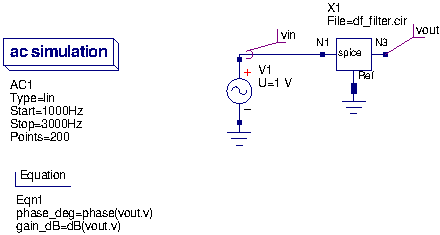
\includegraphics[width=0.6\linewidth]{stoq_fig22}
  \caption{The Dalyiannis-Friend bandpass filter test circuit.}
  \label{fig:stoq_fig22}
\end{figure} 

\begin{figure}
  \centering
  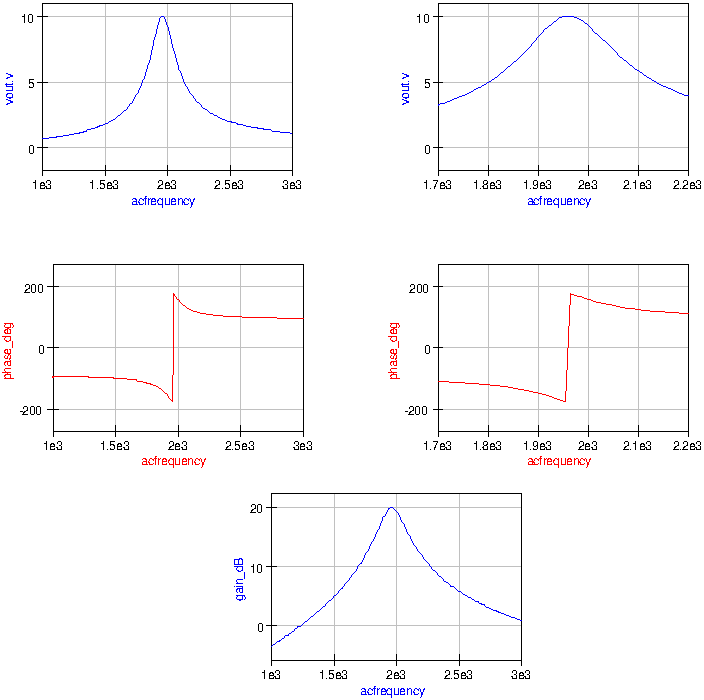
\includegraphics[width=0.6\linewidth]{stoq_fig23}
  \caption{Simulated small signal AC transfer functions for the Dalyiannis-Friend bandpass filter.}
  \label{fig:stoq_fig23}
\end{figure} 

\tutsection{Global nodes}
In the SPICE 2 and SPICE 3 hardware description languages only the earth node is global. By convention this is given node name 0 and is assumed by the SPICE language passer to be earth whenever it occurs in a circuit netlist. When connecting discreet components with other subcircuit blocks there is often a need for other nodes to be designated global; the classic example being power supply nodes.  SPICEPP allows nodes to designated as global. These are effectively connected together to form one net covering both outside and inside subcircuits.  The best way to understand the use of global nodes is to consider an example. Figure~\ref{fig:stoq_fig11} gives the SPICE netlist for the two section CMOS ring counter. Many readers would possibly have noticed that in this netlist both the NAND2 and NOR2 subcircuits include internal voltage sources\footnote{The DC voltage supply for each logic block is generated by a pulse source. This has the effect of simulating the rising edge of the power supply switch on transient and aids DC convergence.}. This is, of course, not necessary and indeed inefficient from a simulation point of view. A better approach would be to link individual gates with a power supply net.  The SPICEPP netlist given in Fig.~\ref{fig:stoq_fig24} illustrates how the .global command can be used to define a global power supply node.  After passing this code through SPICEPP the SPICE netlist printed in Fig.~\ref{fig:stoq_fig25} results. Simulation with Qucs gives the same waveforms displayed in Fig.~\ref{fig:stoq_fig13}.
 
\begin{figure}
 \begin{lstlisting} [
   basicstyle=\scriptsize]   
* Two stage CMOS ring counter circuit.
*
* External nodes: input 1, output 4, +ve supply  nvcc
*
*global node
*
.global nvcc
*
x1 1 5 6  nand2
x2 1 6 7  nand2
x3 3 6 2  nand2
x4 2 7 3  nand2
x5 1 2 8  nor2
x6 1 8 9  nor2
x7 5 8 4  nor2
x8 4 9 5  nor2
*
.model modp pmos( vto=-1 kp=10u
+                         cgdo=0.2n cgso=0.2n cgbo=2n)
.model modn nmos(vto=1 kp=10u
+                         cgdo=0.2n cgso=0.2n cgbo=2n)
*
.subckt nand2 1 2 3 
m1 3 1 nvcc nvcc modp w=40u l=5u
m2 3 2 nvcc nvcc modp w=40u l=5u
m3 5 1 0 0 modn w=20u l=5u
m4 3 2 5 5 modn w=20u l=5u
c1 1 0 10p
c2 2 0 10p
*vcc 4 0 pulse ( 0 5 0 1ns 1ns 1 2)
.ends
*
.subckt nor2 1 2 3
m1 4 1 nvcc nvcc modp w=40u l=5u
m2 3 2 4 4 modp w=40u l=5u
m3 3 2 0 0 modn w=20u l=5u
m4 3 1 0 0 modn w=20u l=5u
c1 1 0 10p
c2 2 0 10p
*vcc 7 0 pulse ( 0 5 0 1ns 1ns 1 2)
.ends
\end{lstlisting} 
 \caption{SPICEPP netlist for a two section CMOS ring counter with global power supply net node nvcc.}
\label{fig:stoq_fig24}
\end{figure}   

\begin{figure}
 \begin{lstlisting} [
   basicstyle=\scriptsize]   
* Two stage CMOS ring counter circuit.
x1 1 5 6 nvcc nand2
x2 1 6 7 nvcc nand2
x3 3 6 2 nvcc nand2
x4 2 7 3 nvcc nand2
x5 1 2 8 nvcc nor2
x6 1 8 9 nvcc nor2
x7 5 8 4 nvcc nor2
x8 4 9 5 nvcc nor2
.model modp pmos vto=-1 kp=10u cgdo=0.2n cgso=0.2n cgbo=2n
.model modn nmos vto=1 kp=10u cgdo=0.2n cgso=0.2n cgbo=2n
.subckt nand2 1 2 3 nvcc
m1 3 1 nvcc nvcc modp w=40u l=5u
m2 3 2 nvcc nvcc modp w=40u l=5u
m3 5 1 0 0 modn w=20u l=5u
m4 3 2 5 5 modn w=20u l=5u
c1 1 0 10p
c2 2 0 10p
.ends
.subckt nor2 1 2 3 nvcc
m1 4 1 nvcc nvcc modp w=40u l=5u
m2 3 2 4 4 modp w=40u l=5u
m3 3 2 0 0 modn w=20u l=5u
m4 3 1 0 0 modn w=20u l=5u
c1 1 0 10p
c2 2 0 10p
.ends
\end{lstlisting} 
 \caption{SPICE netlist for a two section CMOS ring counter with global power supply net node nvcc.}
\label{fig:stoq_fig25}
\end{figure}   

\tutsection{End Note}
This tutorial note describes how SPICE netlists can be simulated using Qucs. The text is much more than a basic outline of the processes needed to link SPICE circuit files to Qucs. While writing this note an attempt has been made to stress the fact that topics like SPICE/Qucs netlist compatibility and conversion are important to the future development of Qucs. So an interesting, and thought provoking question, is how does Qucs develop next in relation to SPICE and indeed how best is it to make sure that Qucs users can get the most from all the published SPICE information and device models?  After all there is no point in reinventing the wheel!  Complete compatibility with SPICE will not be possible until all the basic SPICE 2 and SPICE 3 primitive components are added to Qucs.  This will take time but is happening as the Qucs team develops the package\footnote{Michael Magraf has recently added a four terminal transmission line to Qucs. Future testing will confirm if this is similar to the SPICE T component.}.  Adding equations to component calculations is a very much a current active topic in Qucs development.  Recently, Michael Magraf has added parameter passing to the Qucs GUI. Stefan Jahn will add the necessary simulator routines for handling equations and parameter passing when time allows. In the long term not only will it be possible to determine component values using calculations at the simulation initialisation phase but it will also be possible to allow such components to be dependent on simulation voltage and current variables. Qucs will then be able to simulate circuits containing nonlinear voltage and current sources like the SPICE 3 B component.  These notes are very much a report on some of the work on Qucs device modelling I have been doing in recent months.  Again if there is enough interest in this area of Qucs development I will upgrade them in the future.  My thanks to Stefan Jahn for all his encouragement while I have been developing the material reported in this tutorial note.

